\documentclass[a4paper, 12pt, final, garamond]{book}
\usepackage{cours-preambule}

\raggedbottom

\makeatletter
\renewcommand{\@chapapp}{M\'ecanique -- chapitre}
\makeatother

\begin{document}
\setcounter{chapter}{4}

\chapter{TD entra\^inement~: mouvement de particules charg\'ees}

\section{Séparation isotopique}

Le spectromètre de \textsc{Dempster} permet, entre autres, de séparer les
différents isotopes chargés d'un élément dans un échantillon. \bigbreak

\begin{minipage}{0.50\linewidth}
    Considérons un faisceau de particules chargées, constitué des ions de deux
    isotopes de mercure~: $\ce{^200_80Hg\plus{2}}$ et $\ce{^202_80Hg\plus{2}}$,
    notés respectivement (1) et (2). Ce faisceau sort de la chambre d'ionisation
    avec une vitesse négligeable, puis accéléré par une tension $U_{PP'}$
    appliquée entre les deux plaques $P$ et $P'$. Les ions traversent ensuite
    une zone de déviation où règne un champ magnétique transversal uniforme, tel
    que $\Bf = B\uz$. \bigbreak
\end{minipage}
\hfill
\begin{minipage}{0.50\linewidth}
    \begin{center}
        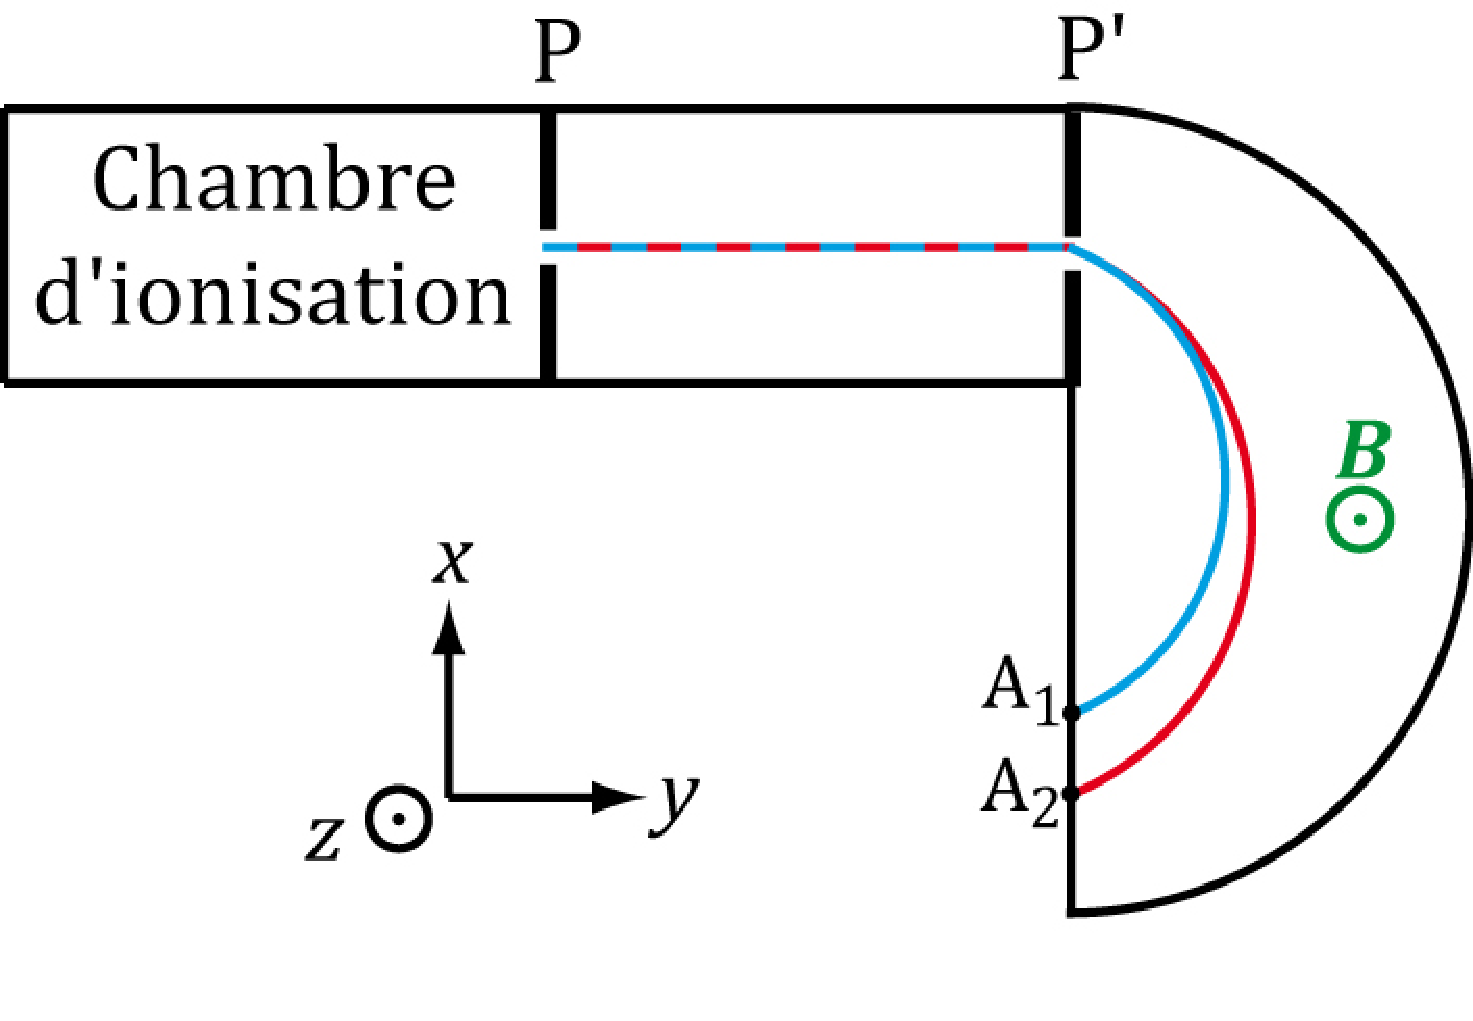
\includegraphics[width=6cm]{dempster}
        \captionof{figure}{Schéma du dispositif}
        \label{fig:dempster}
    \end{center}
\end{minipage}

On donne~: $m\ind{nucléon} = \SI{1.67e-27}{kg}$, $m\ind{électron}$ négligeable
devant $m\ind{nucléon}$, $\abs{U_{PP'}} = \SI{10}{kV}$, $B = \SI{0.10}{T}$ et $e
= \SI{1.6e-19}{C}$. \bigbreak

\begin{enumerate}
    \item Quel doit être le signe de $U_{PP'}$ pour que les ions soient
        effectivement accélérés entre $P$ et $P'$~?
    \item Exprimer les vitesses $v_1$ et $v_2$ des isotopes suite à
        l'accélération.
    \item Déterminer les trajectoires des ions dans la zone de déviation.
        Exprimer les rayons $R_1$ et $R_2$ des trajectoires.
    \item On recueille les particules sur une plaque photographique sous $P'$
        après leur demi-tour. Exprimer puis calculer la distance $d$ entre les
        deux traces observées.
\end{enumerate}

\section{Cyclotron \hfill {\small Inspiré CCP PC 2014, oral banque PT}}
Un cyclotron est formé de deux enceintes demi-cylindriques $D_1$ et $d_2$,
appelées \textit{dees} en anglais, séparées d'une zone étroite d'épaisseur $a$.
Les \textit{dees} sont situés dans l'entrefer d'un électroaimant qui fournit un
champ magnétique uniforme $\Bf = B\ez$, de norme $B = \SI{1.5}{T}$. Une tension
sinusoïdale d'amplitude $U_m = \SI{200}{kV}$ est appliquée entre les deux
extrémités de la bande intermédiaire, si bien qu'il y règne en champ électrique
orienté selon $\ex$. \bigbreak

On injecte des protons de masse $m = \SI{1.7e-27}{kg}$ au sein de la zone
intermédiaire avec une vitesse initiale négligeable. \bigbreak

\begin{minipage}{0.45\linewidth}
    \begin{center}
        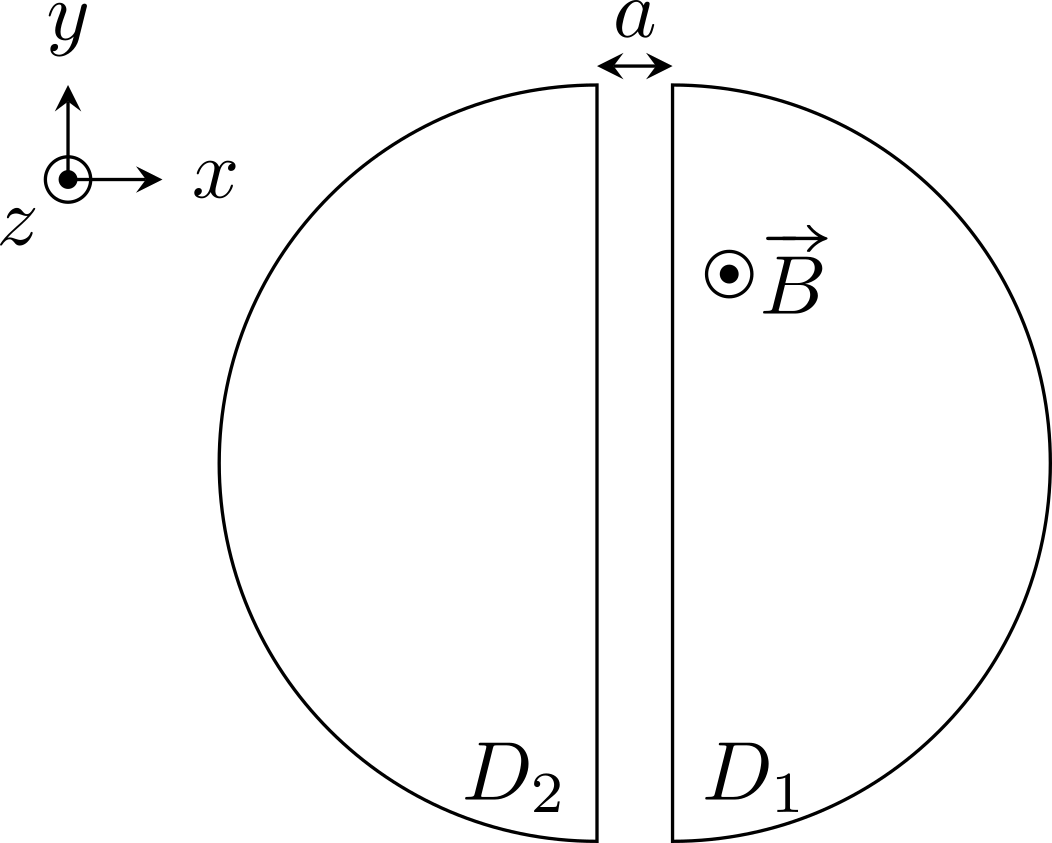
\includegraphics[width=5cm]{cyclotron_exo}
        \captionof{figure}{Schéma de principe.}
        \label{fig:cyclo_exo}
    \end{center}
\end{minipage}
\hfill
\begin{minipage}{0.45\linewidth}
    \begin{center}
        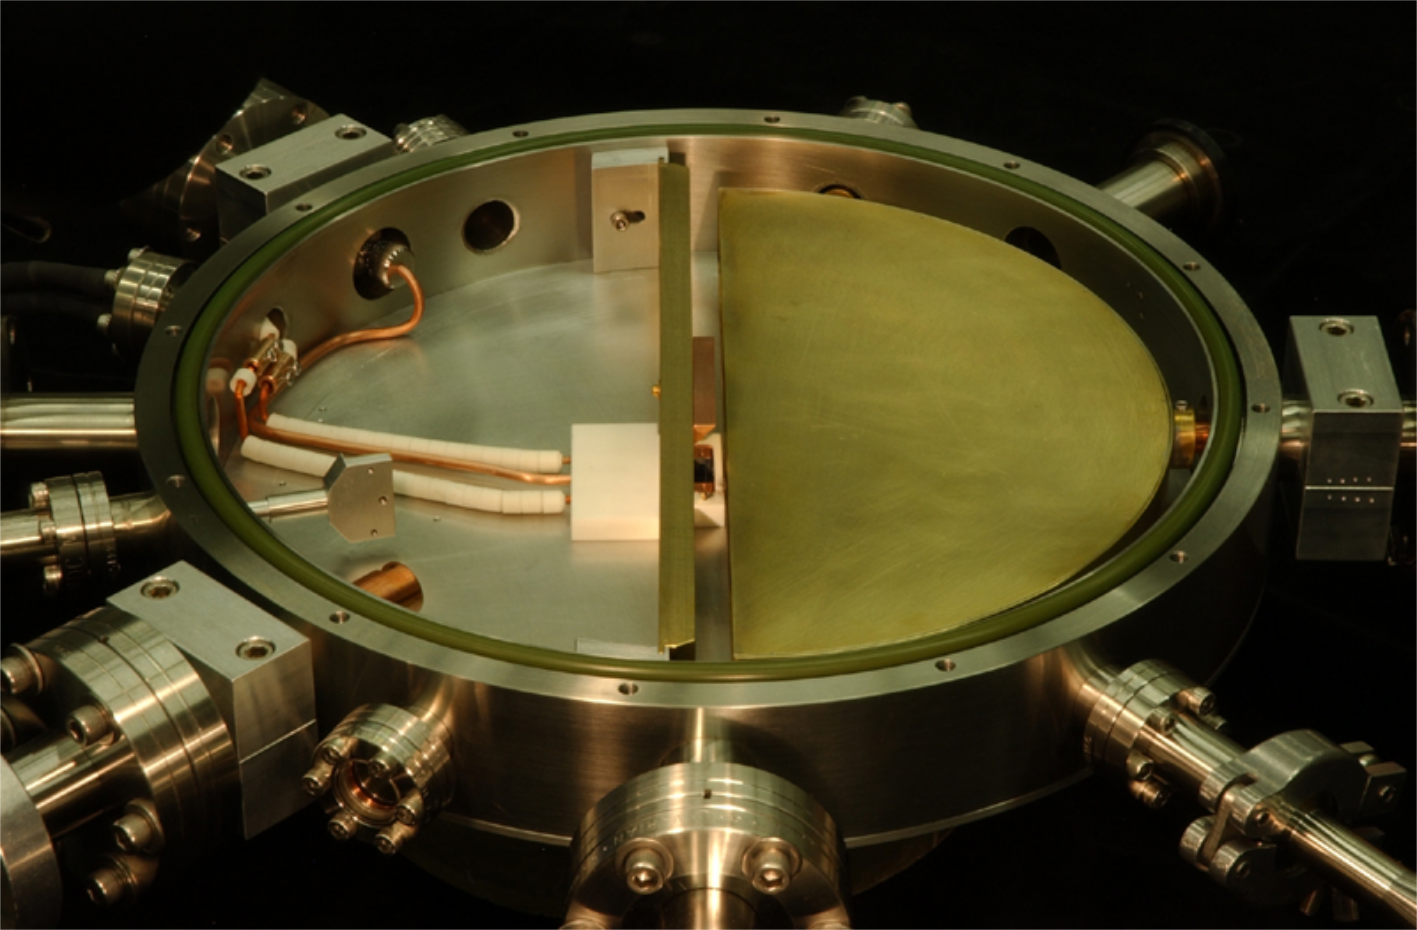
\includegraphics[width=5cm]{cyclotron_rutgers}
        \captionof{figure}{Photon du cyclotron de l'université de
        \textsc{Rutgers}, mesurant $\approx \SI{30}{cm}$ en diamètre.}
        \label{fig:rutgers}
    \end{center}
\end{minipage} \bigbreak

\begin{enumerate}
    \item Montrer qu'à l'intérieur d'un \textit{dee}, la norme de la vitesse des
        protons est constante.
    \item En déduire le rayon de courbure $R$ de la trajectoire des protons
        ayant une vitesse $v$ ainsi que le temps que passe un proton dans un
        \textit{dee}.
    \item Quelle doit être la fréquence $f$ de la tension pour que le proton
        soit accéléré de façon optimale à chaque passage entre les \textit{dee}~?
        Pour simplifier on pourra supposer $a \ll R$. Justifier le choix d'une
        tension harmonique au lieu, par exemple, d'une tension créneau.
    \item Exprimer en fonction de $n$ la vitesse $v_n$ puis le rayon $R_n$ de la
        trajectoire d'un proton après $n$ passages dans la zone d'accélération.
        Le demi-cercle $n=1$ est celui qui suit la première phase
        d'accélération.
    \item Calculer numériquement le rayon de la trajectoire après un tour (donc un
        passage dans chaque \textit{dee}), puis après dix tours.
\end{enumerate} \bigbreak

Le rayon de la dernière trajectoire décrite par les protons accélérés avant de
bombarder une cible est $R_N = \SI{35}{cm}$. \bigbreak

\begin{enumerate}[resume]
    \item Déterminer l'énergie cinétique du proton avant le choc contre la cible
        proche du cyclotron, puis le nombre de tours parcourus par le proton.
\end{enumerate}

\section{Chambre à bulles}

La chambre à bulles est un dispositif mis au point en 1952 par Donald Arthur
\textsc{Glaser} (prix \textsc{Nobel} 1960), et destiné à visualiser des
trajectoires de particules subatomiques. Il s'agit d'une enceinte remplie d'un
liquide (généralement du dihydrogène) à une température légèrement supérieure à
celle de vaporisation~: le passage d'une particule chargée déclenche la
vaporisation et les petites bulles formées ainsi matérialisent la trajectoire de
la particule. \bigbreak

L'ensemble est plongé dans un champ magnétique uniforme et
stationnaire, qui courbe les trajectoires et permet ainsi d'identifier les
particules (à partir de leur masse et de leur charge). \bigbreak

On étudie ici une particule P de masse $m$, de charge $q$ (positive ou
négative), introduite à $t = 0$ dans la chambre à bulles où règne le champ $\Bf
= B \ez$ (avec $B > 0$). Sa position initiale est l'origine O du repère, et sa
vitesse initiale est $\vfo = v_0\ey$ (avec $v_0 > 0$). Le poids de la particule
est négligé dans tout le problème. Le référentiel du laboratoire est supposé
galiléen. \bigbreak

\textit{Dans un premier temps, on suppose que les frottements du liquide sur la
particule P sont négligeables.} \bigbreak

\begin{enumerate}
    \item Établir les équations différentielles du mouvement de P. On posera $\w
        = qB/m$.
    \item En déduire les équations horaires de P et indiquer précisément la
        nature de sa trajectoire. Représenter sur un même schéma les
        trajectoires d'un proton (charge $q = +e$ et masse $m_p$) et d'un
        électron ($q = −e$ et $m_e \ll m_p$).
\end{enumerate} \bigbreak

\textit{Les frottements du liquide sont maintenant modélisés par la force $\Ff =
-\lb\vf_{P}$ avec $\lb$ une constante positive. On pose $\a = \lb/m$.} \bigbreak

\begin{enumerate}[resume]
    \item Établir les nouvelles équations différentielles du mouvement (avec les
        paramètres $\w$ et $\a$). Montrer que le mouvement reste plan.

    \item Déterminer complètement les équations horaires de P. On pourra poser
        la variable complexe $\uu = x + \jj y$, et déterminer tout d'abord
        $\ul{\dot{u}}$.

    \item Déterminer les coordonnées du point asymptotique ${\rm P}_{+\infty} =
        {\rm P}(t \ra \infty)$. Représenter sur un schéma la trajectoire d'un
        proton.
\end{enumerate}

\end{document}
